\documentclass[conference]{IEEEtran}

\usepackage[T1]{fontenc}
\usepackage[utf8]{inputenc}
\usepackage{amsmath,amssymb}
\usepackage{graphicx}
\usepackage{booktabs}
\usepackage{array}
\usepackage{cite}
\usepackage{url}
\usepackage{microtype}
\usepackage[table]{xcolor}
\usepackage{tikz}
\usetikzlibrary{arrows.meta,positioning,calc}

\graphicspath{{./}{../figures/}}
\setlength{\textfloatsep}{6pt plus 1pt minus 2pt}
\setlength{\floatsep}{5pt plus 1pt minus 2pt}
\setlength{\intextsep}{5pt plus 1pt minus 2pt}
\setlength{\abovecaptionskip}{3pt}
\setlength{\belowcaptionskip}{2pt}
\setlength{\parskip}{0pt}

\definecolor{pmuBlue}{HTML}{1D4ED8}
\definecolor{softBlue}{HTML}{DBEAFE}
\definecolor{softGreen}{HTML}{DCFCE7}
\definecolor{softOrange}{HTML}{FFEDD5}
\definecolor{softRed}{HTML}{FEE2E2}
\definecolor{gridGray}{HTML}{64748B}

\title{PI-HED: Physics-Guided Evidence Routing for Sparse-PMU Event Diagnosis on the IEEE 39-Bus System}

\author{
\IEEEauthorblockN{Jorge Luis Mayorga Taborda\IEEEauthorrefmark{1}, Yessica Africano Rodriguez\IEEEauthorrefmark{1}, David Celita\IEEEauthorrefmark{2}, and Masoud Barati\IEEEauthorrefmark{3}}
\IEEEauthorblockA{\IEEEauthorrefmark{1}Universidad de los Andes, Bogota, Colombia\\
\IEEEauthorrefmark{2}Universidad de La Sabana, Chia, Colombia\\
\IEEEauthorrefmark{3}University of Pittsburgh, Pittsburgh, PA, USA}
}

\begin{document}
\maketitle

\begin{abstract}
Sparse phasor measurement unit (PMU) deployments turn event diagnosis into a typed inverse problem: the system must detect an abnormal window, distinguish physical disturbances from measurement-integrity events, and localize a BUS, LINE, PMU, or NONE target from a limited spatial footprint. This paper presents PI-HED, a physics-guided hierarchical evidence decomposition for the IEEE 39-bus system with eight observed PMUs. Each 30~s multi-PMU window is converted into auditable evidence: baseline-relative phasor deviations, onset and persistence statistics, sequence and proxy-power consistency, RLS/Kalman innovation summaries, data-quality indicators, and $Z_{\mathrm{bus}}$-weighted graph-temporal compatibility. A compact ExtraTrees hierarchy then separates physical events from missing/bad-data artifacts and routes each decision to the proper typed localizer. The selected graph-temporal representation improves RAW0001 localization from 0.5000 to 0.6667 while preserving simulation Top-1 localization at 0.8524. The full runtime obtains 0.9693 detection accuracy and 0.9598 event-classification macro-F1 on a 1500-window simulation holdout; on the 21-window RAW0001 transfer folder it matches all observed detection and event labels and reaches 0.6667 Top-1 localization. The result is a reproducible conference-scale bridge between raw PMU machine learning and future multi-hypothesis physical observers.
\end{abstract}

\begin{IEEEkeywords}
synchrophasors, phasor measurement units, event diagnosis, event localization, smart grids, IEEE 39-bus system, physics-informed machine learning.
\end{IEEEkeywords}

\section{Introduction}
Synchrophasor event diagnosis is not a single-label classification problem; it is a coupled inference problem over grid state, event type, sensor integrity, and event location. PMUs measure synchronized voltage and current phasors, frequency, and rate of change of frequency (ROCOF), enabling wide-area monitoring applications \cite{phadke2008,c37118}. In practice, however, only a sparse subset of buses is instrumented. The classifier must therefore infer whether the grid is abnormal, identify the physical or measurement event, and localize the origin from a partial spatial footprint.

This case study targets the IEEE 39-bus system with eight observed PMUs. The data include physical disturbances such as faults, line outages, generation changes, and load changes, together with missing-data and bad-data events. A purely physical estimator would be attractive, but raw PMU streams contain drift, missing samples, timestamp mismatches, channel-specific artifacts, and uncertain event parameters. A purely data-driven model, in contrast, risks learning bus identities and dataset-specific shortcuts rather than electrical behavior. Our approach uses machine learning only after converting each window into a physics-aware representation.

The central idea is to ask a physical question before creating each feature family: how large was the response, how fast did it begin, how persistent was it, whether it was coherent across phases, whether it followed a smooth local trajectory, and whether its spatial pattern was consistent with the network topology. These questions produce robust segment statistics, derivatives, sequence and power-proxy features, recursive innovations, and graph-temporal quantities. A hierarchical ExtraTrees ensemble \cite{geurts2006} then uses the resulting feature row to perform detection, event classification, and typed localization.

The paper makes four contributions. First, it formulates sparse-PMU diagnosis as a typed inverse problem rather than a flat label assignment. Second, it introduces PI-HED, a physics-guided evidence map that turns local residuals, measurement integrity, and electrical-distance compatibility into a single deployable feature row. Third, it evaluates a simulation-trained runtime while treating RAW0001 only as a small transfer-validation folder, not as a training source. Fourth, it compares the selected representation against production-feasible residual and topology variants, while explicitly separating valid transfer evidence from oracle or RAW-label-tuned experiments.

\section{Positioning and Design Principle}
\label{sec:positioning}
Classical power-system state estimation starts from a measurement model and estimates a system state that is consistent with network equations \cite{schweppe1970}. Dynamic state estimation extends this idea by adding machine and controller dynamics, often through Kalman-filter variants \cite{kalman1960,kundur1994}; hybrid symbolic-numeric modeling pushes the same physical agenda into modern computational frameworks \cite{cui2021}. These methods provide an attractive physical interpretation, but they require a sufficiently specified dynamic model, trusted parameters, and enough observability for the state and disturbance being inferred. In the present setting, the available data are sparse PMU files, the disturbance parameters are not supplied, and the raw files include measurement faults that are themselves part of the target taxonomy.

Recent PMU learning methods move in the opposite direction: they map measured waveforms directly to event or location labels using convolutional or recurrent models \cite{li2018,zhu2018}. Related system-identification work learns synchrophasor dynamics with uncertainty-aware models \cite{jalali2021}. These approaches can be powerful when large labeled corpora, stable sensor layouts, or explicit model equations are available, but they are vulnerable to two problems in this case study. First, a fixed neural tensor representation can accidentally encode bus identity and file-layout assumptions. Second, a high-capacity model may fit simulated waveforms while learning little about why a disturbance should propagate through the network in a particular spatial pattern.

The method in this paper is deliberately placed between those two extremes. It is not a full dynamic observer, because it does not solve a nonlinear network model at each time step. It is also not feature extraction followed by generic machine learning. The representation is organized around a small set of physical tests: local abnormality, onset speed, persistence, phase coherence, frequency and power-balance movement, measurement integrity, and electrical-distance consistency. The ExtraTrees layer is used as a nonparametric decision rule over those tests. This design keeps the runtime reproducible while still explaining why the selected evidence should transfer from simulation to raw PMU files.

\section{Data, Topology, and Task}
\label{sec:data}
The case study follows the SGSMA 2026 synchrophasor diagnosis specification \cite{sgsma2026} on the IEEE 39-bus network with a 100~MVA, 60~Hz base. The topology artifacts contain 39 buses, 46 physical branches, the complex admittance matrix $Y_{\mathrm{bus}}$, a pseudoinverse-based $Z_{\mathrm{bus}}$, and effective impedance distances. The observed PMUs are located at buses 2, 5, 6, 10, 19, 22, 29, and 39. The simulation corpus contains 5000 labeled windows, split into 3500 training windows and a 1500-window stratified holdout; 1186 holdout windows are abnormal and therefore localizable. RAW0001 is a separate 21-window transfer folder with 9 normal and 12 abnormal windows. Fig.~\ref{fig:pmumap} shows the sparse observation pattern.

\begin{figure*}[t]
\centering
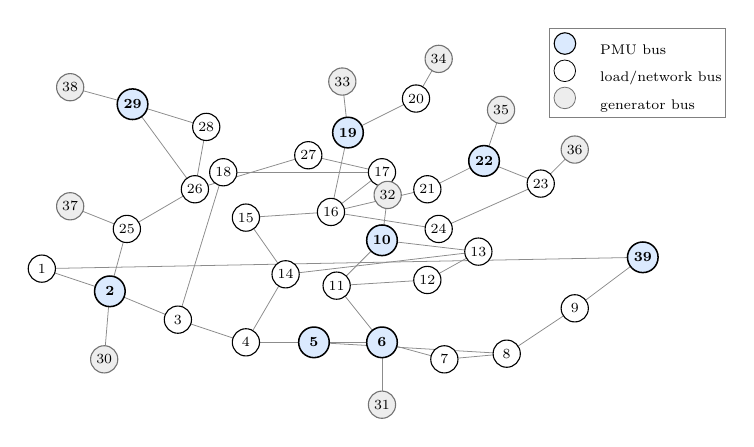
\begin{tikzpicture}[scale=0.72, transform shape,
  bus/.style={circle,draw=black,fill=white,inner sep=1.1pt,font=\scriptsize,minimum size=4.8mm},
  pmu/.style={circle,draw=black,fill=softBlue,line width=0.55pt,inner sep=1.1pt,font=\scriptsize\bfseries,minimum size=5.4mm},
  gen/.style={circle,draw=black!55,fill=black!7,inner sep=1.0pt,font=\scriptsize,minimum size=4.8mm},
  branch/.style={draw=black!45,line width=0.28pt},
  legendbox/.style={rectangle,draw=black!50,fill=white,inner sep=2pt,font=\scriptsize}
]
\coordinate (c1) at (0.0,2.8);   \coordinate (c2) at (1.2,2.4);
\coordinate (c3) at (2.4,1.9);   \coordinate (c4) at (3.6,1.5);
\coordinate (c5) at (4.8,1.5);   \coordinate (c6) at (6.0,1.5);
\coordinate (c7) at (7.1,1.2);   \coordinate (c8) at (8.2,1.3);
\coordinate (c9) at (9.4,2.1);   \coordinate (c10) at (6.0,3.3);
\coordinate (c11) at (5.2,2.5);  \coordinate (c12) at (6.8,2.6);
\coordinate (c13) at (7.7,3.1);  \coordinate (c14) at (4.3,2.7);
\coordinate (c15) at (3.6,3.7);  \coordinate (c16) at (5.1,3.8);
\coordinate (c17) at (6.0,4.5);  \coordinate (c18) at (3.2,4.5);
\coordinate (c19) at (5.4,5.2);  \coordinate (c20) at (6.6,5.8);
\coordinate (c21) at (6.8,4.2);  \coordinate (c22) at (7.8,4.7);
\coordinate (c23) at (8.8,4.3);  \coordinate (c24) at (7.0,3.5);
\coordinate (c25) at (1.5,3.5);  \coordinate (c26) at (2.7,4.2);
\coordinate (c27) at (4.7,4.8);  \coordinate (c28) at (2.9,5.3);
\coordinate (c29) at (1.6,5.7);  \coordinate (c30) at (1.1,1.2);
\coordinate (c31) at (6.0,0.4);  \coordinate (c32) at (6.1,4.1);
\coordinate (c33) at (5.3,6.1);  \coordinate (c34) at (7.0,6.5);
\coordinate (c35) at (8.1,5.6);  \coordinate (c36) at (9.4,4.9);
\coordinate (c37) at (0.5,3.9);  \coordinate (c38) at (0.5,6.0);
\coordinate (c39) at (10.6,3.0);

\foreach \a/\b in {
1/2,1/39,10/32,11/10,11/12,11/6,12/13,13/10,14/13,14/4,
15/14,15/16,16/17,16/19,17/18,18/3,19/20,19/33,2/25,2/30,
20/34,21/16,22/21,22/23,22/35,23/24,23/36,24/16,25/26,25/37,
26/28,27/17,27/26,29/26,29/28,29/38,3/2,4/3,4/5,5/6,
5/8,6/31,6/7,7/8,8/9,9/39}
  \draw[branch] (c\a) -- (c\b);
\foreach \n in {1,3,4,7,8,9,11,12,13,14,15,16,17,18,20,21,23,24,25,26,27,28}
  \node[bus] at (c\n) {\n};
\foreach \n in {30,31,32,33,34,35,36,37,38}
  \node[gen] at (c\n) {\n};
\foreach \n in {2,5,6,10,19,22,29,39}
  \node[pmu] at (c\n) {\n};
\node[legendbox,anchor=west] at (8.95,6.25) {
  \begin{tabular}{@{}ll@{}}
  \tikz{\node[pmu,minimum size=3.8mm,inner sep=0.5pt]{};} & PMU bus\\
  \tikz{\node[bus,minimum size=3.8mm,inner sep=0.5pt]{};} & load/network bus\\
  \tikz{\node[gen,minimum size=3.8mm,inner sep=0.5pt]{};} & generator bus
  \end{tabular}
};
\end{tikzpicture}
\caption{Schematic IEEE 39-bus topology and PMU placement used in the case study. Edges follow the 46 physical branches; highlighted buses are observed by PMUs.}
\label{fig:pmumap}
\end{figure*}

\subsection{Sparse PMU Observation Model}
Each PMU file contains timestamped three-phase voltage and current magnitudes and angles, frequency, ROCOF, and data-presence fields. The runtime sorts each file independently and uses 30~s windows. Row-consistent windowing is preferred for raw files because timestamp drift across PMU CSVs can create artificial missingness if the files are outer-merged on floating-point timestamps.

The sparse layout matters. With only eight observed buses, the algorithm cannot assume that the event origin is directly instrumented. A fault at an unobserved bus, a line outage between two unobserved buses, or a remote generation/load change is only visible through the response induced at the PMU buses. The learning problem is therefore closer to sparse inverse diagnosis than to direct sensor classification: the model must infer an event and a location from a projected spatial-temporal footprint. This motivates graph-relative features and typed localizers instead of a single global label predictor.

\subsection{Labels and Output Contract}

The event taxonomy is shown in Table~\ref{tab:taxonomy}. Events 1--4 correspond to physical grid disturbances, events 5--7 correspond to data-quality or measurement phenomena, and event 8 represents mixed or unknown physical evidence. This taxonomy motivates a hierarchical model: missing and bad-data evidence should not be forced into the same flat classifier as physical grid events.

\begin{table}[t]
\centering
\caption{Event taxonomy and dominant evidence.}
\label{tab:taxonomy}
\renewcommand{\arraystretch}{1.06}
\footnotesize
\begin{tabular}{@{}cll@{}}
\toprule
\textbf{Id} & \textbf{Event} & \textbf{Dominant evidence} \\
\midrule
0 & Normal & baseline consistency \\
1 & Fault & voltage sag, derivative, severity pattern \\
2 & Line outage & current redistribution, graph pair differences \\
3 & Generation & frequency/ROCOF and power-proxy shift \\
4 & Load & sustained current and power-proxy movement \\
5 & Missing data & gaps, NaNs, low data-present fraction \\
6 & Missing + physical & data-quality loss plus physical evidence \\
7 & Bad data & isolated channel/PMU inconsistency \\
8 & Unknown/mixed & physical evidence with low class confidence \\
\bottomrule
\end{tabular}
\end{table}

Table~\ref{tab:eventsignatures} gives the compact physical signature used to interpret each non-normal event. The table is not a list of hard decision rules for the final model; it is the engineering rationale used to build and audit the feature set. This distinction is important because real PMU windows often contain weak evidence across several blocks. The tree ensemble combines those weak cues, while the table keeps the model accountable to a physical story.

\begin{table*}[t]
\centering
\caption{Compact physical signatures used to design and audit the event features.}
\label{tab:eventsignatures}
\renewcommand{\arraystretch}{1.08}
\footnotesize
\begin{tabular}{@{}p{0.12\textwidth}p{0.34\textwidth}p{0.46\textwidth}@{}}
\toprule
\textbf{Event} & \textbf{Expected PMU footprint} & \textbf{Feature evidence used by the model} \\
\midrule
Fault & Abrupt voltage depression, large derivative, localized severity gradient, possible phase imbalance. & Voltage span and early deltas, derivative energy, robust-$z$ peak, sustained anomaly, sequence/phase-coherence features, graph timing and candidate scores. \\
Line outage & Current redistribution with weaker voltage shock than a fault; pairwise PMU changes reveal the affected corridor. & Current span, current-angle movement, rolling current energy, pairwise PMU differences, weighted graph differences, LINE-specific localizer candidates. \\
Generation event & System-wide frequency and ROCOF response with sustained power-balance movement. & Late frequency shift, ROCOF span, $P/Q$ proxy movement, RLS/Kalman innovation timing, BUS localizer over generation/load candidate buses. \\
Load event & Sustained current and proxy-power shift, often less impulsive than a fault. & Late current deltas, proxy $P$ shift, rolling energy, smooth-residual features, graph spread across nearby PMUs. \\
Missing data & Data-present fraction drops, NaNs or timestamp gaps dominate the evidence. & Data-quality counters, missing-run statistics, PMU-level availability ratios, missing-composition detector. \\
Bad data & A single PMU or channel breaks local consistency without a coherent network response. & Single-signal abnormality ratio, isolated robust-$z$ spike, phase-inconsistency features, bad-data detector and PMU localizer. \\
Mixed/unknown & Physical evidence exists but event-specific confidence is low or conflicting. & Low event-margin, high entropy, competing fault/outage/generation/load features, graph residual mismatch. \\
\bottomrule
\end{tabular}
\end{table*}

\section{Method}
\label{sec:method}
Fig.~\ref{fig:method} summarizes the model. The pipeline first turns raw PMU tensors into one feature row per 30~s window. Three decision modules then score the row: a physical event classifier for events 0, 1, 2, 3, 4, and 8; a missing-data detector for events 5 and 6; and a bad-data detector for event 7. A rule layer resolves high-risk confusion cases, and the final event is routed to a typed localizer.

PI-HED can be read as a discriminative approximation to a physical posterior. For a window $Y_k$ and network graph $\mathcal{G}$, the desired decision is
\begin{equation}
(\hat e_k,\hat \tau_k,\hat \ell_k)=
\arg\max_{e,\tau,\ell}p(e,\tau,\ell\mid Y_k,\mathcal{G}),
\end{equation}
where $e$ is the event, $\tau\in\{\mathrm{BUS},\mathrm{LINE},\mathrm{PMU},\mathrm{NONE}\}$ is the target type, and $\ell$ is the target object. The implemented model replaces a full multi-hypothesis observer with
\begin{equation}
p(e,\tau,\ell\mid Y_k,\mathcal{G})\approx p_\theta(e,\tau,\ell\mid \Phi(Y_k,\mathcal{G})),
\end{equation}
where $\Phi$ is an auditable evidence map rather than an unconstrained raw waveform embedding.
The routing layer also enforces the output contract: normal windows map to NONE, faults/generation/load changes map to BUS candidates, line outages map to LINE candidates, and missing or bad-data events map to PMU candidates. This removes impossible label combinations before the localizer is asked to rank targets.

\begin{figure}[t]
\centering
\resizebox{\columnwidth}{!}{%
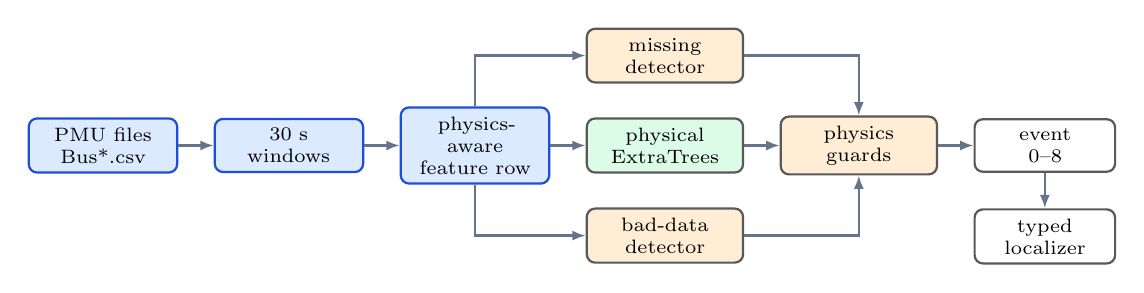
\begin{tikzpicture}[
  node distance=0.45cm and 0.45cm,
  box/.style={rounded corners=3pt,draw=pmuBlue,fill=softBlue,thick,text width=1.65cm,minimum height=0.56cm,align=center,font=\scriptsize},
  phys/.style={rounded corners=3pt,draw=black!65,fill=softGreen,thick,text width=1.75cm,minimum height=0.56cm,align=center,font=\scriptsize},
  guard/.style={rounded corners=3pt,draw=black!65,fill=softOrange,thick,text width=1.75cm,minimum height=0.56cm,align=center,font=\scriptsize},
  outbox/.style={rounded corners=3pt,draw=black!65,fill=white,thick,text width=1.55cm,minimum height=0.56cm,align=center,font=\scriptsize},
  arrow/.style={-{Latex[length=1.7mm]},draw=gridGray,thick}
]
\node[box] (raw) {PMU files\\Bus*.csv};
\node[box,right=of raw] (win) {30 s\\windows};
\node[box,right=of win] (feat) {physics-aware\\feature row};
\node[phys,right=of feat] (clf) {physical\\ExtraTrees};
\node[guard,above=0.43cm of clf] (miss) {missing\\detector};
\node[guard,below=0.43cm of clf] (bad) {bad-data\\detector};
\node[guard,right=of clf] (rules) {physics\\guards};
\node[outbox,right=of rules] (event) {event\\0--8};
\node[outbox,below=0.45cm of event] (loc) {typed\\localizer};
\draw[arrow] (raw) -- (win);
\draw[arrow] (win) -- (feat);
\draw[arrow] (feat) -- (clf);
\draw[arrow] (feat) |- (miss);
\draw[arrow] (feat) |- (bad);
\draw[arrow] (clf) -- (rules);
\draw[arrow] (miss) -| (rules);
\draw[arrow] (bad) -| (rules);
\draw[arrow] (rules) -- (event);
\draw[arrow] (event) -- (loc);
\end{tikzpicture}
}
\caption{Runtime architecture. A single feature row is shared by physical, missing-data, and bad-data models; the event output is then routed to a typed location model.}
\label{fig:method}
\end{figure}

\subsection{Local Baseline and Robust Abnormality}
All electrical features are relative to a local pre-event baseline. For PMU $p$, signal $s$, and windowed signal $x_{p,s}(t)$, the robust abnormality score is
\begin{equation}
z_{p,s}(t)=
\frac{x_{p,s}(t)-\mathrm{median}(x_{p,s}^{\mathrm{pre}})}
{1.4826\,\mathrm{MAD}(x_{p,s}^{\mathrm{pre}})+\epsilon}.
\end{equation}
The extractor computes segment statistics over pre, early, mid, late, and full-window intervals. The early segment captures onset shock, the mid segment captures transient settling, and the late segment captures persistent operating-point movement. Derivative features,
\begin{equation}
d_x(t)=\frac{x(t)-x(t-\Delta t)}{\Delta t},
\end{equation}
capture abrupt faults, switching behavior, and corrupted samples. Sustained robust-$z$ features distinguish a physical deviation that persists from an isolated bad-data spike.

\subsection{Physics-Aware Feature Families}
Table~\ref{tab:features} maps each feature block to its physical role. The base block includes voltage/current magnitude and angle statistics, robust deviations, derivatives, three-phase consistency, and positive/negative/zero-sequence quantities. A power-proxy block uses normalized phasor magnitudes and angle separation to compute
\begin{equation}
\begin{aligned}
P_{\mathrm{proxy}}&=V_{pu}I_{pu}\cos(\theta_V-\theta_I),\\
Q_{\mathrm{proxy}}&=V_{pu}I_{pu}\sin(\theta_V-\theta_I),
\end{aligned}
\end{equation}
which is not a calibrated power-flow measurement but gives the classifier a stable active/reactive movement signature.

\begin{table*}[t]
\centering
\caption{Feature blocks, physical question, and event signature.}
\label{tab:features}
\renewcommand{\arraystretch}{1.08}
\footnotesize
\begin{tabular}{@{}p{0.18\textwidth}p{0.31\textwidth}p{0.43\textwidth}@{}}
\toprule
\textbf{Feature block} & \textbf{Physical question} & \textbf{Event-diagnosis role} \\
\midrule
Segment statistics and deltas & How large and persistent is the response relative to the pre window? & Faults create large early deviations; load/generation changes often appear as sustained late shifts. \\
Derivatives and rolling energy & How fast does the signal move, and over which time scale? & Voltage derivatives support fault detection; current derivatives and rolling energy support outage and switching signatures. \\
Robust $z$ and sustained anomaly & Is the deviation large relative to local noise, and does it persist? & Sustained abnormality supports physical events; isolated high-$z$ channels support bad-data routing. \\
Sequence and phase consistency & Is the three-phase structure physically coherent? & Real grid events tend to preserve structured phase relationships; corrupted channels break local coherence. \\
Data quality and single-signal ratio & Is the evidence caused by unavailable data or one inconsistent channel? & Missing and bad-data events are routed before physical labels to avoid contaminating event 1--4 decisions. \\
Power proxy and frequency/ROCOF & Does the window show balance or inertia-related motion? & Generation and load changes are better explained by sustained frequency, ROCOF, and proxy $P/Q$ movement than by a voltage sag alone. \\
RLS/Kalman innovations & Does the signal break from a smooth local trajectory? & Adaptive residuals detect abrupt departures while ignoring smooth ramps and local drift. \\
Graph-temporal features & Does the spatial response match electrical proximity and PMU-pair timing? & Line outages and localized faults benefit from pairwise PMU differences weighted by electrical distance. \\
\bottomrule
\end{tabular}
\end{table*}

\subsection{Adaptive and Graph-Temporal Features}
The selected dynamic block adds rolling windows of 5, 15, 30, 60, and 120 samples and recursive residual features on representative voltage, current, angle, frequency, and ROCOF signals. A recursive least-squares level/linear predictor and a scalar Kalman level model produce residual and innovation summaries such as maximum residual, mean residual, 95th percentile, late-pre delta, and time to peak. These features answer whether the signal can be explained by a smooth local trajectory or whether an event has broken that trajectory.

The graph-temporal block uses the effective impedance distance
\begin{equation}
d_Z(i,j)=\left|Z_{ii}+Z_{jj}-Z_{ij}-Z_{ji}\right|
\end{equation}
and pairwise PMU differences. For a candidate event origin $i$, the method also forms a diffusion-like kernel over observed PMUs:
\begin{equation}
k_i(p;\tau)=\exp\left(-d_Z(p,i)/\tau\right).
\end{equation}
If $a_p$ is a scalar severity score at observed PMU $p$, candidate compatibility is summarized by
\begin{equation}
c_i(\tau)=
\frac{\sum_p a_p k_i(p;\tau)}
{\left(\sum_p a_p^2\right)^{1/2}
 \left(\sum_p k_i(p;\tau)^2\right)^{1/2}+\epsilon}.
\end{equation}
The resulting features include candidate scores, margins, entropies, residuals, weighted PMU differences, pairwise correlations, and time-to-peak differences.

The important modeling choice is that localization is typed. A fault, generator change, or load change is localized over bus candidates; a line outage is localized over line candidates; a missing or bad-data event is localized over PMU candidates. This avoids forcing a line identifier, bus identifier, and PMU identifier into one incompatible target space. For a line candidate $(i,j)$, the graph features summarize the response near both terminal buses and the contrast between PMUs electrically close to one side versus the other. For a PMU candidate, the localizer emphasizes single-instrument inconsistency and data-quality evidence rather than network propagation.

This candidate construction gives the model a weak form of physical hypothesis testing. Each candidate produces a set of compatibility features, but the final probability is learned from data. The method therefore does not require specifying exact event impedances, dropped load sizes, generator inertia constants, or protection-clearing times. It only requires the weaker assumption that nearby electrical locations should leave more similar PMU footprints than distant locations, and that physical events should be more spatially coherent than isolated data artifacts.

\subsection{Hierarchical ExtraTrees Decision Layer}
Each decision model is a median imputer followed by a scikit-learn ExtraTrees classifier \cite{geurts2006,pedregosa2011}. ExtraTrees are appropriate here because the input is high-dimensional, heterogeneous, and threshold-heavy: missing-data fractions, robust deviations, derivative magnitudes, graph scores, and localizer candidate features do not require the same scale. Four supervised targets are trained from the same engineered feature rows: the physical event label, a bad-data indicator, a missing-composition label, and typed location labels. The route is intentionally not a single flat classifier. Missing-only windows route to event 5 and a PMU localizer; bad-data windows route to event 7 and a PMU localizer; physical events route to BUS or LINE localizers depending on the event type and predicted target space.

\begin{table}[t]
\centering
\caption{Runtime inference sequence.}
\label{tab:runtime}
\renewcommand{\arraystretch}{1.08}
\footnotesize
\begin{tabular}{@{}cp{0.78\columnwidth}@{}}
\toprule
\textbf{Step} & \textbf{Operation} \\
\midrule
1 & Discover PMUs from input filenames and validate required PMU columns. \\
2 & Sort each PMU stream and form row-consistent 30~s windows. \\
3 & Compute baseline-relative, dynamic, data-quality, and graph-temporal features. \\
4 & Apply imputation and hierarchical ExtraTrees event routing. \\
5 & Route to BUS, LINE, or PMU localizer and keep Top-3 candidates in diagnostics. \\
6 & Expand the window decision back to timestamp--bus rows for the required CSV. \\
\bottomrule
\end{tabular}
\end{table}

\section{Training and Feature Selection}
\label{sec:training}
Training used the simulated scenario set with a 30\% stratified holdout for validation. RAW0001 was used as a transfer validation set rather than a training source for the final model. This distinction is important: exploratory variants that fit or weight RAW labels can improve RAW0001 numbers but are not valid evidence of generalization to a new raw folder.

\begin{table}[t]
\centering
\caption{Validity controls used during model selection.}
\label{tab:safeguards}
\renewcommand{\arraystretch}{1.05}
\footnotesize
\begin{tabular}{@{}p{0.36\columnwidth}p{0.55\columnwidth}@{}}
\toprule
\textbf{Validity risk} & \textbf{Control used in this paper} \\
\midrule
RAW memorization & Train feature statistics, imputers, thresholds, and trees on simulation only. \\
PMU layout shortcut & Discover PMU buses from filenames and encode topology-relative evidence. \\
Oracle localization & Reject candidate promotion that uses true RAW event labels or ranks. \\
Metric cherry-picking & Select the final path by preserving SIM performance and improving frozen RAW transfer. \\
Measurement artifacts & Route missing and bad-data events before physical BUS/LINE localization. \\
\bottomrule
\end{tabular}
\end{table}

The model-selection criterion was therefore two-sided. A candidate feature set had to preserve simulation performance, because the simulation holdout is the only broad labeled source, and it also had to improve RAW0001 transfer behavior without using RAW0001 labels for training. We report localization progression because localization is the most sensitive task: detection can be solved by large abnormality scores, while localization requires that the spatial pattern be assigned to the right bus, line, or PMU target.

All feature stages preserve the same inference contract and model family. The changes in Fig.~\ref{fig:trainingprogress} are therefore attributable to representation, not to a different learning algorithm. The selected stage contains 45,162 structured features: repeated physical summaries across PMU, phase, signal, segment, and candidate dimensions. The training seed is fixed at 20260503; the ExtraTrees hierarchy uses median imputation, balanced class weights where applicable, 650--750 trees, and the same 30~s windows for all variants.

Fig.~\ref{fig:trainingprogress} and Table~\ref{tab:ablation} show the feature-stage progression for localization. The base representation already performs strongly on simulation, but RAW localization is weak. Rolling features produce a small simulation gain but do not change RAW. RLS/Kalman residuals improve RAW by capturing dynamic departures from a smooth trajectory. The graph-temporal block gives the selected model its best deployable balance: 0.8524 SIM Top-1 and 0.6667 RAW0001 Top-1. Table~\ref{tab:alternatives} gives the adversarial sanity check: when the same general-purpose tree families are trained on dynamic window statistics without the PI-HED evidence map and typed routing, RAW transfer collapses. The comparison is not meant to claim neural-network superiority; it isolates the value of physics-structured evidence under the same sparse-PMU data constraints.

\begin{figure}[t]
\centering
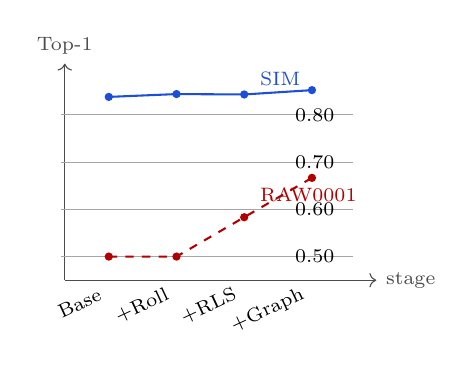
\begin{tikzpicture}[x=0.86cm,y=1cm,font=\scriptsize]
\draw[->,black!70] (0,0) -- (4.6,0) node[right] {stage};
\draw[->,black!70] (0,0) -- (0,2.75) node[above] {Top-1};
\foreach \y/\lab in {0.30/0.50,0.90/0.60,1.50/0.70,2.10/0.80}
  \draw[black!35] (-0.05,\y) -- (4.25,\y) node[left=3pt,black] {\lab};
\foreach \x/\lab in {0.65/Base,1.65/+Roll,2.65/+RLS,3.65/+Graph}
  \node[rotate=25,anchor=east] at (\x,-0.12) {\lab};
\draw[pmuBlue,line width=0.75pt] (0.65,2.328) -- (1.65,2.364) -- (2.65,2.359) -- (3.65,2.414);
\draw[red!70!black,line width=0.75pt,dashed] (0.65,0.30) -- (1.65,0.30) -- (2.65,0.80) -- (3.65,1.30);
\foreach \x/\y in {0.65/2.328,1.65/2.364,2.65/2.359,3.65/2.414}
  \fill[pmuBlue] (\x,\y) circle (1.5pt);
\foreach \x/\y in {0.65/0.30,1.65/0.30,2.65/0.80,3.65/1.30}
  \fill[red!70!black] (\x,\y) circle (1.5pt);
\node[anchor=west,pmuBlue] at (2.74,2.56) {SIM};
\node[anchor=west,red!70!black] at (2.74,1.08) {RAW0001};
\end{tikzpicture}
\caption{Localization progression during feature selection. Dynamic residuals and graph-temporal features improve transfer validation on RAW0001 while preserving simulation performance.}
\label{fig:trainingprogress}
\end{figure}

\begin{table}[t]
\centering
\caption{Localization feature-stage progression.}
\label{tab:ablation}
\renewcommand{\arraystretch}{1.08}
\footnotesize
\begin{tabular}{@{}p{0.30\columnwidth}rcc@{}}
\toprule
\textbf{Variant} & \textbf{\#feat.} & \textbf{SIM} & \textbf{RAW} \\
\midrule
\texttt{base\_v2} & 39,744 & 0.8381 & 0.5000 \\
+ rolling & 43,104 & 0.8440 & 0.5000 \\
+ RLS/Kalman & 44,448 & 0.8432 & 0.5833 \\
+ graph-temporal & 45,162 & 0.8524 & 0.6667 \\
\bottomrule
\end{tabular}
\end{table}

\begin{table}[t]
\centering
\caption{Sanity baselines against generic dynamic-feature ML.}
\label{tab:alternatives}
\renewcommand{\arraystretch}{1.05}
\scriptsize
\begin{tabular}{@{}p{0.30\columnwidth}cccc@{}}
\toprule
\textbf{Method} & \textbf{SIM F1} & \textbf{SIM L} & \textbf{RAW D} & \textbf{RAW L} \\
\midrule
Dyn. RF & 0.7619 & 0.4628 & 0.5714 & 0.0833 \\
Dyn. ET & 0.7633 & 0.4587 & 0.5714 & 0.0000 \\
PI-HED & \textbf{0.9598} & \textbf{0.8524} & \textbf{1.0000} & \textbf{0.6667} \\
\bottomrule
\end{tabular}
\end{table}

\section{Results}
\label{sec:results}
Table~\ref{tab:metrics} reports the final selected-model results, and Fig.~\ref{fig:metriclines} visualizes the same task-level pattern. Detection and event classification are strong on both validation splits. Localization is the harder task because multiple physical origins can produce similar sparse PMU footprints, especially with only eight observed buses. On the simulation holdout, exact localization varies strongly by event family: line outages and generation changes are easiest (0.9247 and 0.9777), load changes and bad-data locations remain harder (0.7378 and 0.6104), and event 8 is deliberately difficult because it represents mixed or unknown physical evidence. Wilson intervals quantify the remaining uncertainty: SIM localization is 1011/1186, 95\% CI [0.831, 0.871], while RAW0001 localization is 8/12, 95\% CI [0.391, 0.862].

\begin{table}[t]
\centering
\caption{Final selected-model validation metrics. RAW0001 is a transfer folder, not a training source.}
\label{tab:metrics}
\renewcommand{\arraystretch}{1.10}
\footnotesize
\begin{tabular}{@{}p{0.48\columnwidth}cc@{}}
\toprule
\textbf{Metric} & \textbf{SIM} & \textbf{RAW0001} \\
\midrule
Detection accuracy & 0.9693 & 1.0000 \\
Event classification accuracy & 0.9673 & 1.0000 \\
Event macro-F1 / observed-class F1 & 0.9598 & 1.0000 \\
Localization Top-1 accuracy & 0.8524 & 0.6667 \\
\bottomrule
\end{tabular}
\end{table}

\begin{figure}[t]
\centering
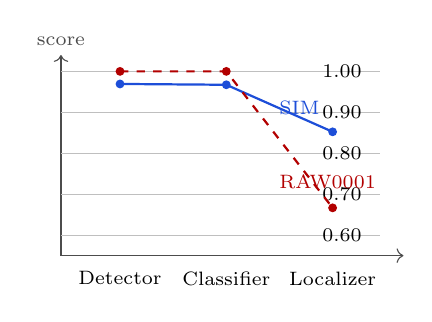
\begin{tikzpicture}[x=1cm,y=5.2cm,font=\scriptsize]
\draw[->,black!70] (0,0.55) -- (0,1.04) node[above] {score};
\draw[->,black!70] (0,0.55) -- (4.35,0.55);
\foreach \y/\lab in {0.60/0.60,0.70/0.70,0.80/0.80,0.90/0.90,1.00/1.00}
  \draw[black!25] (0,\y) -- (4.05,\y) node[left=3pt,black] {\lab};
\foreach \x/\lab in {0.75/Detector,2.10/Classifier,3.45/Localizer}
  \node[anchor=north] at (\x,0.535) {\lab};
\draw[pmuBlue,line width=0.8pt] (0.75,0.9693) -- (2.10,0.9673) -- (3.45,0.8524);
\draw[red!70!black,line width=0.8pt,dashed] (0.75,1.0000) -- (2.10,1.0000) -- (3.45,0.6667);
\foreach \x/\y in {0.75/0.9693,2.10/0.9673,3.45/0.8524}
  \fill[pmuBlue] (\x,\y) circle (1.6pt);
\foreach \x/\y in {0.75/1.0000,2.10/1.0000,3.45/0.6667}
  \fill[red!70!black] (\x,\y) circle (1.6pt);
\node[anchor=west,pmuBlue] at (2.65,0.91) {SIM};
\node[anchor=west,red!70!black] at (2.65,0.73) {RAW0001};
\end{tikzpicture}
\caption{Task-level validation metrics for the selected runtime. The gap between classification and localization is the expected signature of sparse PMU observability: it is easier to determine that an event happened than to identify the exact physical origin.}
\label{fig:metriclines}
\end{figure}

On RAW0001, detection had no false positives or false negatives: 9 normal windows and 12 abnormal windows were correctly separated. Event classification also matched all observed labels; the corresponding 21/21 Wilson lower bound is 0.845. Localization remained imperfect, which is expected under sparse observability: the four missed locations were one line outage (LINE23--24 predicted as LINE22--35), one missing-plus-physical event (BUS2 predicted as LINE2--30), one generation event (BUS2 predicted as BUS38), and one load event (BUS7 predicted as BUS12). The selected features reduce but do not eliminate this ambiguity.

The RAW0001 result should be interpreted carefully. Perfect event classification on a small raw folder does not prove that the classifier will be perfect on all raw folders. Its value is instead diagnostic: the representation learned on simulation did not collapse when applied to a real-file format with raw timing, missingness, and channel artifacts. The more conservative claim is that robust baselines, dynamic residuals, and graph-relative features improved transfer behavior without requiring a raw-label-tuned model.

The final package is CPU-only and does not require a neural-network runtime. It loads a compact model bundle, performs median imputation inside each tree pipeline, and writes a diagnostic JSON file with route, timing, window predictions, and Top-3 location candidates. A local RAW0001 timing check required 823.67~s for 89.65~min of PMU data, or approximately 9.19~s of computation per PMU-data minute on the local Windows CPU environment. The compact archive size is approximately 33~MB, and the local regression/integration/unit test suite reported 246 passing tests and 10 skipped tests.

\section{Discussion and Limitations}
\label{sec:discussion}
The results support a specific lesson: physics-informed features can make a conventional ensemble behave like a structured event-diagnosis system. The model does not receive a raw tensor and discover physics from scratch. It receives features that already encode onset, persistence, cross-phase coherence, data integrity, frequency dynamics, and topology-relative propagation. This representation lets a compact ExtraTrees hierarchy separate physical events from measurement artifacts and route each event to an appropriate target space.

The main limitations are empirical scope and physical depth. RAW0001 is intentionally treated as a small transfer folder, so the result supports representation transfer rather than universal field performance; the PMU-placement stress-test code is implemented, but a full placement sweep is left for the journal extension. The method is also still discriminative: graph features are inspired by the network, but the runtime does not maintain a hidden dynamic state, simulate each candidate event, or explicitly balance PMU measurements against KCL/KVL and swing-equation residuals. The contribution should therefore be read as a high-performing conference method and as a bridge toward a journal extension in which each candidate fault, outage, load change, generation loss, or sensor event is scored by a physical likelihood with measurement, dynamic, topology, and event-parameter residual terms.

\section{Conclusion}
This paper presented PI-HED, a physics-guided PMU event-diagnosis method for the IEEE 39-bus system. The selected model combines bus-agnostic PMU discovery, 30~s windowing, robust baseline-relative features, adaptive residuals, graph-temporal topology features, hierarchical event routing, and typed location models. It achieved strong detection and classification performance and improved RAW localization through dynamic and graph evidence. The broader conclusion is that PMU machine learning should begin with physical questions, not feature volume: what changed, how fast, how persistently, whether the change is coherent, and whether the sparse spatial footprint is plausible on the network.

\begin{thebibliography}{00}

\bibitem{phadke2008}
A. G. Phadke and J. S. Thorp, \emph{Synchronized Phasor Measurements and Their Applications}. New York, NY, USA: Springer, 2008.

\bibitem{c37118}
IEEE Standard for Synchrophasor Measurements for Power Systems, IEEE Std C37.118.1-2011, Dec. 2011.

\bibitem{kalman1960}
R. E. Kalman, ``A new approach to linear filtering and prediction problems,'' \emph{Journal of Basic Engineering}, vol. 82, no. 1, pp. 35--45, Mar. 1960.

\bibitem{schweppe1970}
F. C. Schweppe and J. Wildes, ``Power system static-state estimation, Part I: Exact model,'' \emph{IEEE Transactions on Power Apparatus and Systems}, vol. PAS-89, no. 1, pp. 120--125, Jan. 1970.

\bibitem{kundur1994}
P. Kundur, \emph{Power System Stability and Control}. New York, NY, USA: McGraw-Hill, 1994.

\bibitem{cui2021}
H. Cui, F. Li, and K. Tomsovic, ``Hybrid symbolic-numeric framework for power system modeling and analysis,'' \emph{IEEE Transactions on Power Systems}, vol. 36, no. 2, pp. 1373--1384, Mar. 2021.

\bibitem{li2018}
W. Li, D. Deka, M. Chertkov, and M. Wang, ``Real-time faulted line localization and PMU placement in power systems through convolutional neural networks,'' arXiv:1810.05247, 2018.

\bibitem{zhu2018}
Y. Zhu, C. Liu, and K. Sun, ``Image embedding of PMU data for deep learning towards transient disturbance classification,'' arXiv:1812.09427, 2018.

\bibitem{jalali2021}
M. Jalali, V. Kekatos, S. Bhela, H. Zhu, and V. Centeno, ``Inferring power system dynamics from synchrophasor data using Gaussian processes,'' arXiv:2105.12608, 2021.

\bibitem{geurts2006}
P. Geurts, D. Ernst, and L. Wehenkel, ``Extremely randomized trees,'' \emph{Machine Learning}, vol. 63, no. 1, pp. 3--42, Apr. 2006.

\bibitem{pedregosa2011}
F. Pedregosa \emph{et al.}, ``Scikit-learn: Machine learning in Python,'' \emph{Journal of Machine Learning Research}, vol. 12, pp. 2825--2830, 2011.

\bibitem{sgsma2026}
SGSMA 2026 Synchrophasor Anomaly Detection Competition, ``Competition day policy and submission specification,'' 2026.

\end{thebibliography}

\end{document}
